\documentclass[12pt, a4paper]{article}
\setlength{\textheight}{24cm}
\setlength{\textwidth}{16cm}
\setlength{\topmargin}{0cm}
\setlength{\evensidemargin}{0cm}
\setlength{\oddsidemargin}{0cm}
\usepackage[affil-it]{authblk}
\usepackage{graphics}
\usepackage{graphicx}
\usepackage{caption}
\usepackage{float}
\usepackage[british]{babel}
\usepackage{hyperref}
\usepackage{subcaption}
\date{}
\begin{document}
\title{Comparison of some FFT libraries in C/C++}
\author{Philippe Gambron \thanks{\texttt{philippe.gambron{@}stfc.ac.uk}}, Sue Thorne \thanks{\texttt{sue.thorne{@}stfc.ac.uk}}}
\affil{Science and Technology Facilities Council, Hartree Centre, Rutherford Appleton Laboratory, Harwell Campus, Harwell Oxford, OX11 0QZ, United Kingdom}
\maketitle
\begin{abstract}
We compare the performance of several libraries computing FFTs called from C/C++ code and running on a single node. 
\end{abstract}
\section{Introduction}
Some applications require the computation of the fast Fourier transform (FFT) of large datasets. In such a case, the efficiency of that step can become of critical importance. In this report, we compare the performance obtained with several libraries that can be called from C or C++.
\section{Overview of the chosen libraries}
We consider the following libraries computing FFTs: FFTW \cite{fftw}, MKL \cite{mkl}, GSL \cite{gsl} and FFTPACK \cite{fftpack} (Table \ref{ffttable}). They can perform complex transforms, real-to-half-complex ones (and conversely) as well as, in the case of FFTW, real-to-real transforms when the signal is odd or even. The half-complex output consists in half as many complex values as there were points in the signal, taking advantage of the hermiticity of the Fourier transform of a real function.\\

The GSL and FFTPACK libraries only work in one dimension\footnote{FFTPACK can compute FFTs in several dimensions but it is written in FORTRAN and all the C or C++ wrappers we have found only allowed one-dimensional transforms.}. On the contrary, FFTW and MKL can compute FFTs in several dimensions. They are also capable of working in a parallel way, using multithreading and MPI.  
\begin{table}[H]
\captionsetup{width=1\textwidth}
\begin{tabular}{|p{2.5cm}||p{2.5cm}|p{1cm}|p{3cm}|p{3cm}|p{2cm}|p{2cm}|}
\hline
& Type & Dim. & Radices & Parallelism & Licence \\
\hline
\hline
FFTW & R$\to$H,\ \ \  C$\to$C,\ \ \  H$\to$R, R{\scriptsize (odd/even)}$\to$R& Any&2, 3, 5, 7, 11, 13 + any with code generator & Multithreading, MPI & GPL v2\\
\hline
MKL  &  R$\to$H,\ \ \  C$\to$C,\ \ \ \  H$\to$R& Any & & Multithreading, MPI & Proprietary\\
\hline
GSL  &  R$\to$H,\ \ \  C$\to$C,\ \ \ \  H$\to$R & 1 & 2, 3, 5, 6, 7 & - & GPL v3\\
\hline
FFTPACK {\scriptsize (CASA wrapper)} &  R$\to$H,\ \ \  C$\to$C,\ \ \ \  H$\to$R & 1 & & - & GPL v2\\
\hline
\end{tabular}
\caption{Overview of the FFT libraries considered. R stands for real, C, for complex, and HC, for half-complex.}
\label{ffttable}
\end{table}
\section{Benchmark}
The benchmark \cite{code} consists of calculating the FFT of a series of volumes, in 1, 2 or 3 dimensions, of real or complex values. The purpose was to mimick a problem submitted to us by the CCP PET-MR collaboration \cite{ccppetmr}, within the Software Outlook initiative \cite{softwareoutlook}, who needed to take the transform of a series of square complex images. This example is depicted in Fig. \ref{benchmark} and considered in Section \ref{CCPPETMR}. For our more general test, in Sections \ref{PERFORMANCE1D}, \ref{PERFORMANCE2D} and \ref{PERFORMANCE3D}, the 2-dimensional slices could be replaced by a line or a rectangular cuboid. We used 32 images, which was a typical value used by that collaboration, for the tests that were representative of their requirement. For the other runs, we always processed a single image.\\

\begin{verbatim}
// create a real or complex signal of dimensions N1, N2 ...
// (asymetrical multi-dimensional step function) 
for i running from 0 to N_IMAGES
  image[i]=generate_image({N1, N2 ...})

initialise FFT

for i running from 0 to N_IMAGES
  transform[i]=FFT(image[i])

initialise inverse_FFT

for i running from 0 to N_IMAGES
  inverse_transform[i]=FFT(image[i])

error=sum(||inverse_transform[i]/(N1 N2 ...) - signal[i]||)
\end{verbatim}

We used a number of points varying from $\sim 10^3$ to $\sim 10^7$ in 1, 2 and 3 dimensions. The domains had sides of equal lengths (square or cubic) or were flattened (rectangle or cuboid). These dimensions could be powers of 2, products of powers of small integers (2, 3, 5 and 7) or prime numbers. We used a single thread in all cases except when we assessed the effect of multithreading. In that case, the number of threads was increased till 24.\\

The values appearing in the graphs are the execution time averaged over 10 runs. A certain number of bumps or slight unexpected features are apparent. However they were consistently repeated in all our measurements. This is also confirmed by the standard deviation of our results which was always quite small, of the order of a few percents of the average value. We chose not to display error bars on our graphs since they were so small that they were barely visible. 

\begin{figure}[H]
\captionsetup{width=0.6\textwidth}
\centering
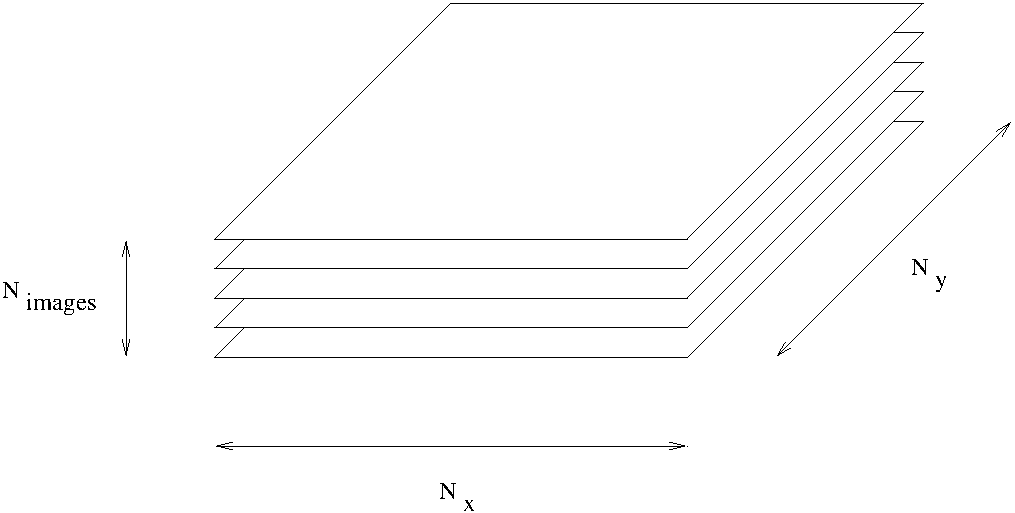
\includegraphics[height=5cm]{benchmark.pdf}
\caption{The benchmark consists in taking the FFT of several images. Each of them is made of real or complex values and can be a simple line, a rectangle or a cuboid.}
\label{benchmark}
\end{figure}

\section{Set up}
Our measurements were carried out on ARCHER \cite{archer}. The modules \texttt{gcc/7.2.0} and \\ \texttt{intel/17.0.3.191} were loaded. In order to take advantage of multi-threading, the environment variable \texttt{KMP\_AFFINITY} must be set to \texttt{disabled}.\\

Our benchmark was coded in C++ using double-precision reals. More precisely, we used version 3.3.8 of FFTW, version 17.0.3 of MKL and version 2.5 of GSL. Note that we used our own version of Boost, FFTW and GSL because the version of Boost present on the system was lacking certain libraries and we wanted to use the most recent versions of FFTW and GSL. The benchmark was compiled with the flags \texttt{-std=c++1z -O3  -fopenmp   -lm -lfftw3 -lfftw3\_threads -lgslcblas -lgsl -lboost\_system -lboost\_chrono -liomp5 -lmkl\_core -lmkl\_intel\_thread \\-lmkl\_intel\_lp64  -lcasa\_scimath  -llapack}.\\

Since FFTPACK was written in FORTRAN, we have resorted to the C++ wrapper provided by CASA, the radioastronomy package \cite{casa}. This is straightforward on Debian-like systems, as the one used by CCP PET-MR in their virtual environment, where CASA can be installed using the package manager. However, including the headers and linking with the libraries was not possible with the version of CASA distributed by the National Radio Astronomy Observatory. As a consequence, this was quite difficult to set up on ARCHER and required the use of libraries provided by an old version of Debian to match those available on the system. For this reason, it was necessary to use as well an older version of CASA, 2.4.0.

\pagebreak
\section{Effect of the domain size for 1D problems}\label{PERFORMANCE1D}

In this section, w compare the performance of each library, for numbers of points consisting of powers of 2, products of powers of small integers and prime numbers. We do so for real and complex values and with FFTW (Fig. \ref{1DFFTWR} and \ref{1DFFTWC}), MKL (Fig. \ref{1DMKLR} and \ref{1DMKLC}), GSL (Fig. \ref{1DGSLR} and \ref{1DGSLC}) and FFTPACK (Fig. \ref{1DFFTPACKR} and \ref{1DFFTPACKC}). We then compare the different libraries for powers of 2 (Fig. \ref{1DPOW2R} and \ref{1DPOW2C}) and in general (Fig. \ref{1DR} and \ref{1DC}).\\



As expected, for all the libraries, the performance is worse with primes than with powers of 2 or products of powers of small integers. According to our measurements, the MKL library tends to be the fastest. We also notice that the performance with primes is significantly worse, with real numbers, in the cases of GSL and FFTPACK.
\begin{figure}[H]
\captionsetup{width=0.8\linewidth}
\centering
\begin{subfigure}{.5\textwidth}
\centering
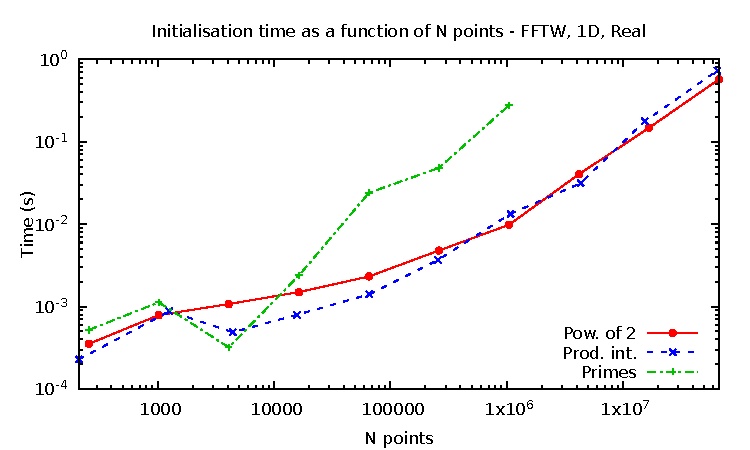
\includegraphics[width=.9\linewidth]{graphs/1d-fftw-init-r.pdf}
\caption{Intialisation (real)}
\label{1DFFTWRI}
\end{subfigure}%
\begin{subfigure}{.5\textwidth}
\centering
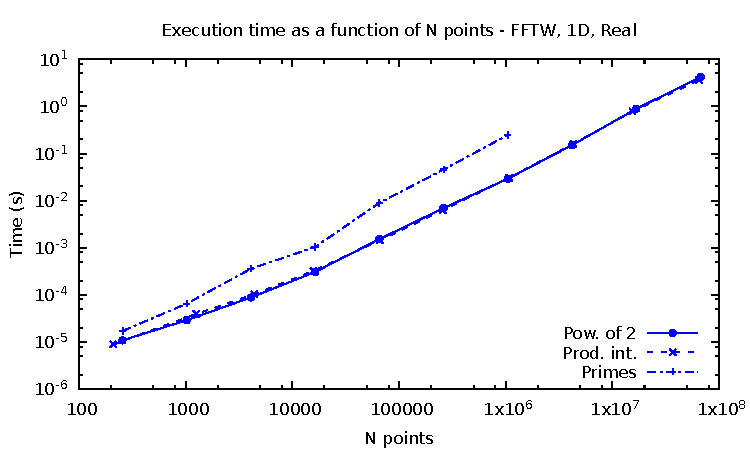
\includegraphics[width=.9\linewidth]{graphs/1d-fftw-exec-r.pdf}
\caption{Execution (real)}
\label{1DFFTWR}
\end{subfigure}\\
\begin{subfigure}{.5\textwidth}
\centering
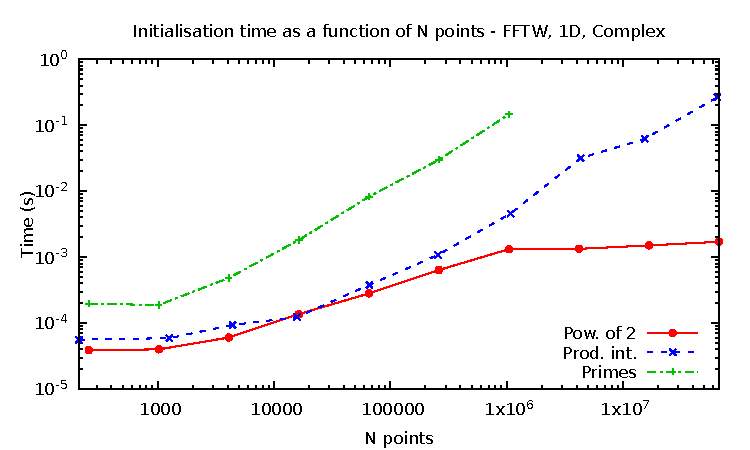
\includegraphics[width=.9\linewidth]{graphs/1d-fftw-init-c.pdf}
\caption{Intialisation (complex)}
\label{1DFFTWCI}
\end{subfigure}%
\begin{subfigure}{.5\textwidth}
\centering
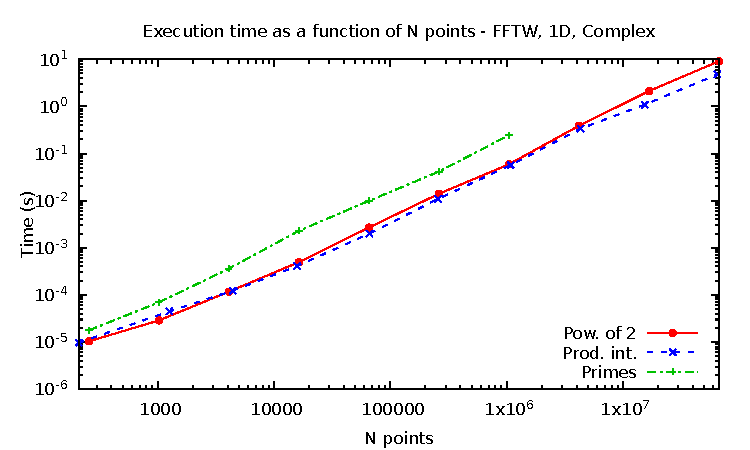
\includegraphics[width=.9\linewidth]{graphs/1d-fftw-exec-c.pdf}
\caption{Execution (complex)}
\label{1DFFTWC}
\end{subfigure}
\caption{Initialisation and execution times as a function of the number of points\\(1 dimension, FFTW, 1 thread)}
\label{1DFFTW}
\end{figure}

\begin{figure}[H]
\captionsetup{width=0.8\linewidth}
\centering
\begin{subfigure}{.5\textwidth}
\centering
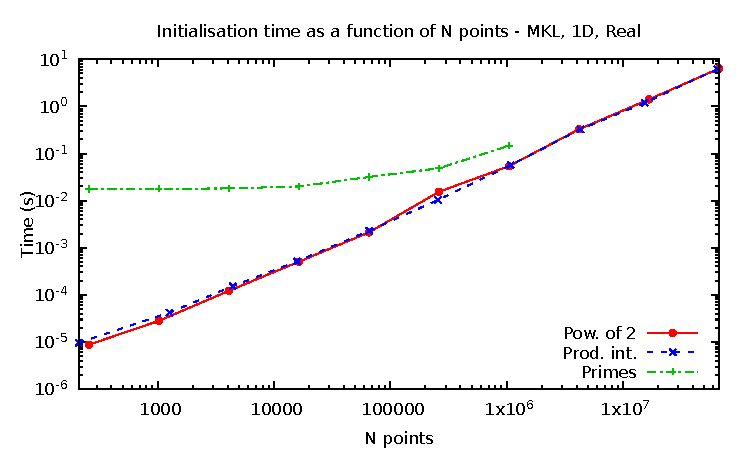
\includegraphics[width=.9\linewidth]{graphs/1d-mkl-init-r.pdf}
\caption{Intialisation (real)}
\label{1DMKLRI}
\end{subfigure}%
\begin{subfigure}{.5\textwidth}
\centering
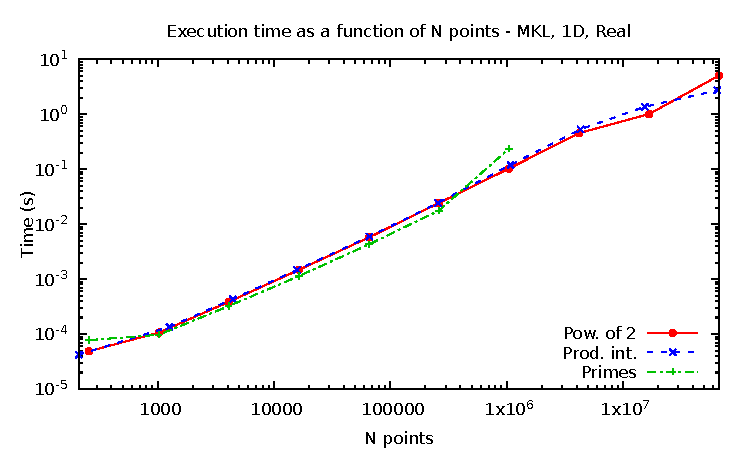
\includegraphics[width=.9\linewidth]{graphs/1d-mkl-exec-r.pdf}
\caption{Execution (real)}
\label{1DMKLR}
\end{subfigure}\\
\begin{subfigure}{.5\textwidth}
\centering
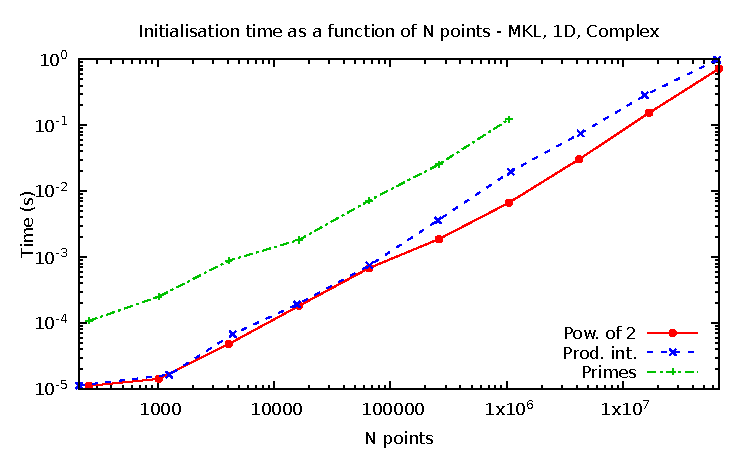
\includegraphics[width=.9\linewidth]{graphs/1d-mkl-init-c.pdf}
\caption{Intialisation (complex)}
\label{1DMKLCI}
\end{subfigure}%
\begin{subfigure}{.5\textwidth}
\centering
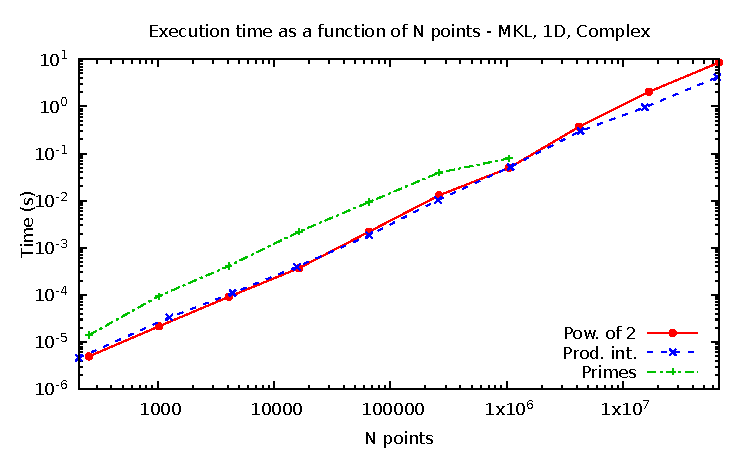
\includegraphics[width=.9\linewidth]{graphs/1d-mkl-exec-c.pdf}
\caption{Execution (complex)}
\label{1DMKLC}
\end{subfigure}\\
\caption{Initialisation and execution times as a function of the number of points\\(1 dimension, MKL, 1 thread)}
\label{1DMKL}
\end{figure}

\begin{figure}[H]
\captionsetup{width=0.8\linewidth}
\centering
\begin{subfigure}{.5\textwidth}
\centering
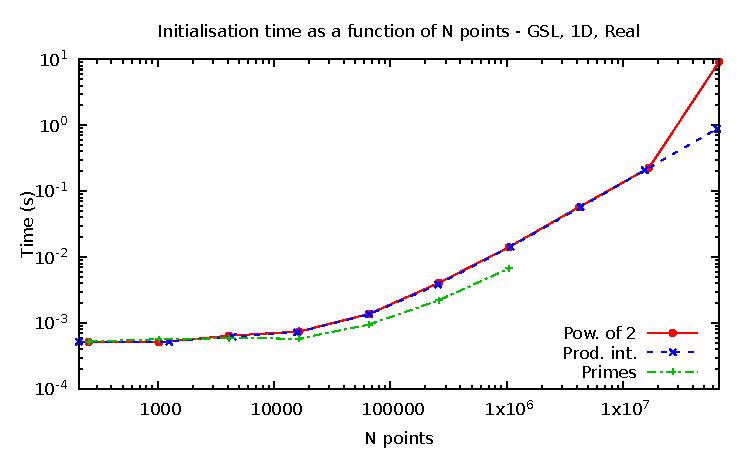
\includegraphics[width=.9\linewidth]{graphs/1d-gsl-init-r.pdf}
\caption{Intialisation (real)}
\label{1DGSLRI}
\end{subfigure}%
\begin{subfigure}{.5\textwidth}
\centering
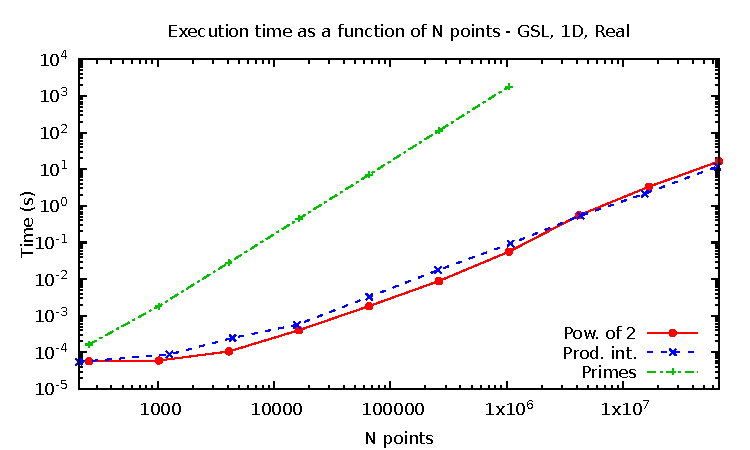
\includegraphics[width=.9\linewidth]{graphs/1d-gsl-exec-r.pdf}
\caption{Execution (real)}
\label{1DGSLR}
\end{subfigure}\\
\begin{subfigure}{.5\textwidth}
\centering
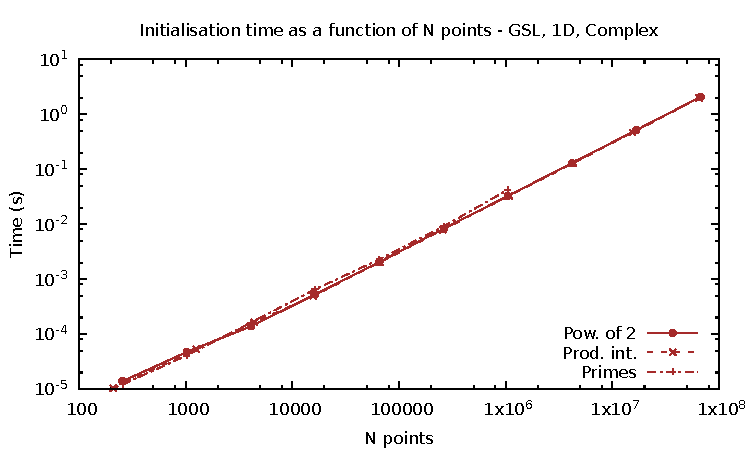
\includegraphics[width=.9\linewidth]{graphs/1d-gsl-init-c.pdf}
\caption{Intialisation (complex)}
\label{1DGSLCI}
\end{subfigure}%
\begin{subfigure}{.5\textwidth}
\centering
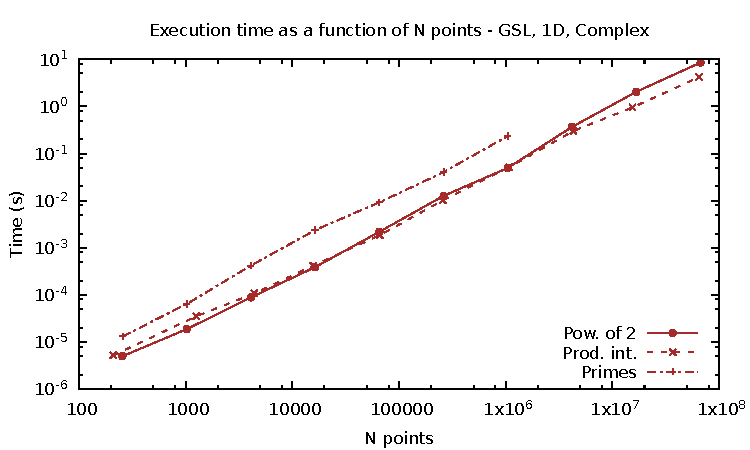
\includegraphics[width=.9\linewidth]{graphs/1d-gsl-exec-c.pdf}
\caption{Execution (complex)}
\label{1DGSLC}
\end{subfigure}
\caption{Initialisation and execution times as a function of the number of points\\(1 dimension, GSL, 1 thread)}
\label{1DGSL}
\end{figure}

\begin{figure}[H]
\captionsetup{width=0.8\linewidth}
\centering
\begin{subfigure}{.5\textwidth}
\centering
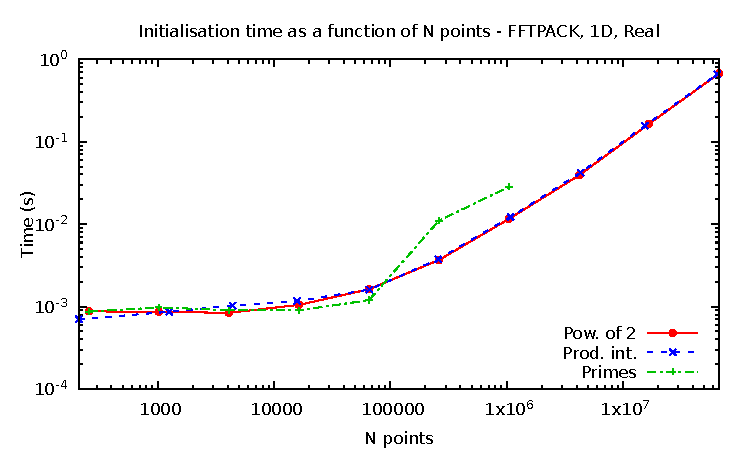
\includegraphics[width=.9\linewidth]{graphs/1d-fftpack-init-r.pdf}
\caption{Intialisation (real)}
\label{1DFFTPACKRI}
\end{subfigure}%
\begin{subfigure}{.5\textwidth}
\centering
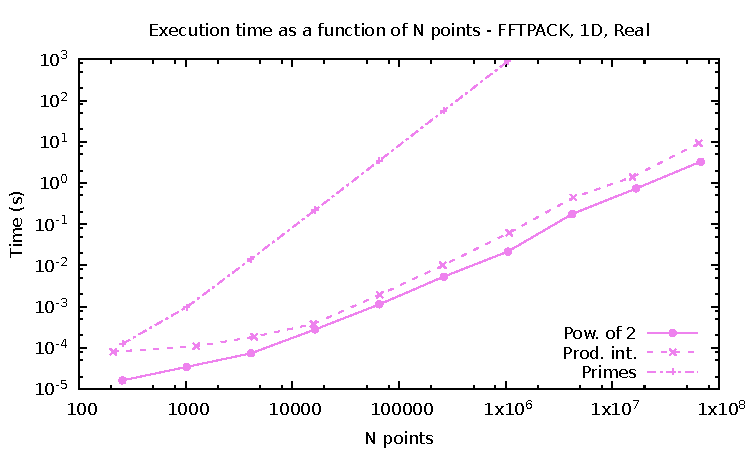
\includegraphics[width=.9\linewidth]{graphs/1d-fftpack-exec-r.pdf}
\caption{Execution (real)}
\label{1DFFTPACKR}
\end{subfigure}\\
\begin{subfigure}{.5\textwidth}
\centering
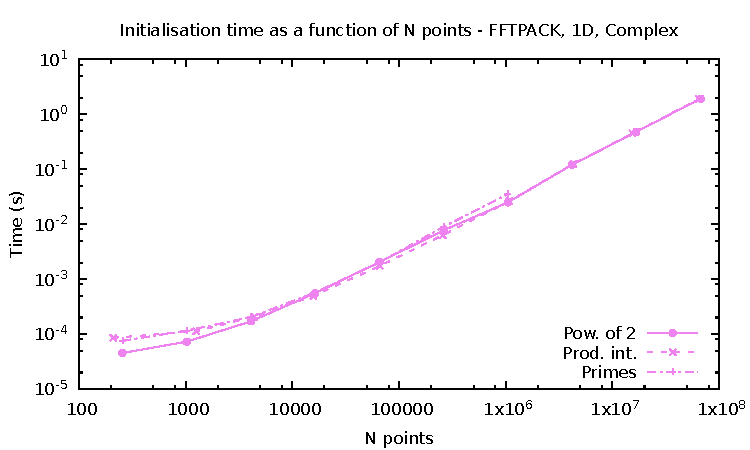
\includegraphics[width=.9\linewidth]{graphs/1d-fftpack-init-c.pdf}
\caption{Intialisation (complex)}
\label{1DFFTPACKCI}
\end{subfigure}%
\begin{subfigure}{.5\textwidth}
\centering
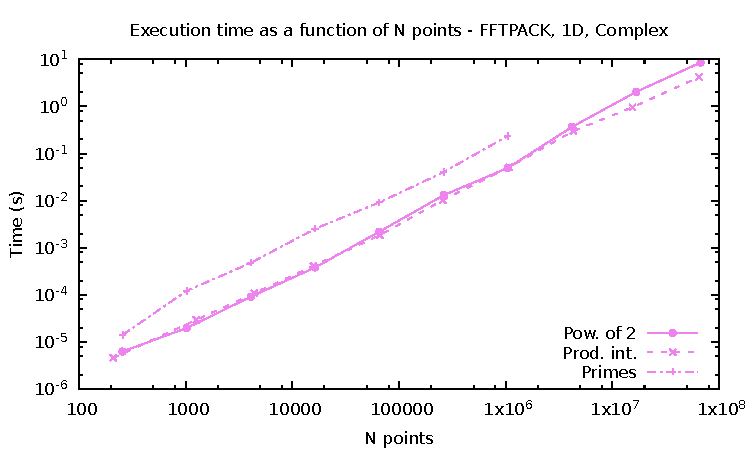
\includegraphics[width=.9\linewidth]{graphs/1d-fftpack-exec-c.pdf}
\caption{Execution (complex)}
\label{1DFFTPACKC}
\end{subfigure}
\caption{Initialisation and execution times as a function of the number of points\\(1 dimension, FFTPACK, 1 thread)}
\label{1DFFTPACK}
\end{figure}

\begin{figure}[H]
\captionsetup{width=0.8\linewidth}
\centering
\begin{subfigure}{.5\textwidth}
\centering
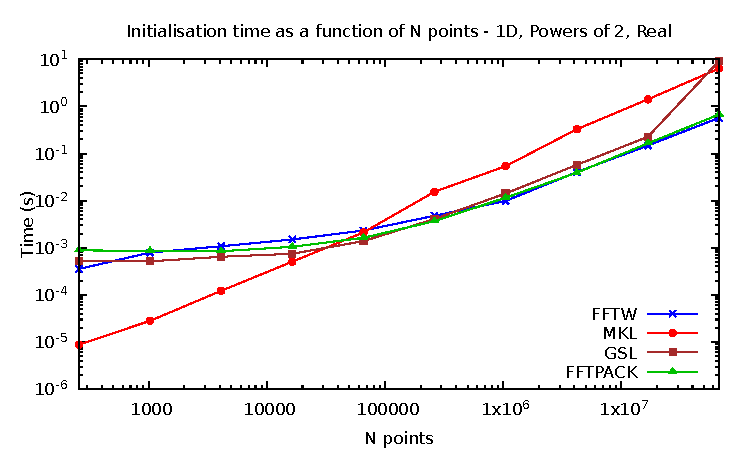
\includegraphics[width=.9\linewidth]{graphs/1d-pow2-init-r.pdf}
\caption{Intialisation (real)}
\label{1DPOW2RI}
\end{subfigure}%
\begin{subfigure}{.5\textwidth}
\centering
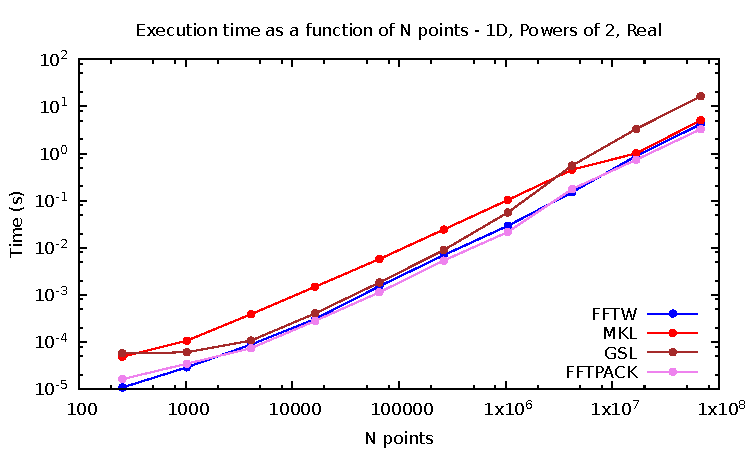
\includegraphics[width=.9\linewidth]{graphs/1d-pow2-exec-r.pdf}
\caption{Execution (real)}
\label{1DPOW2R}
\end{subfigure}\\
\begin{subfigure}{.5\textwidth}
\centering
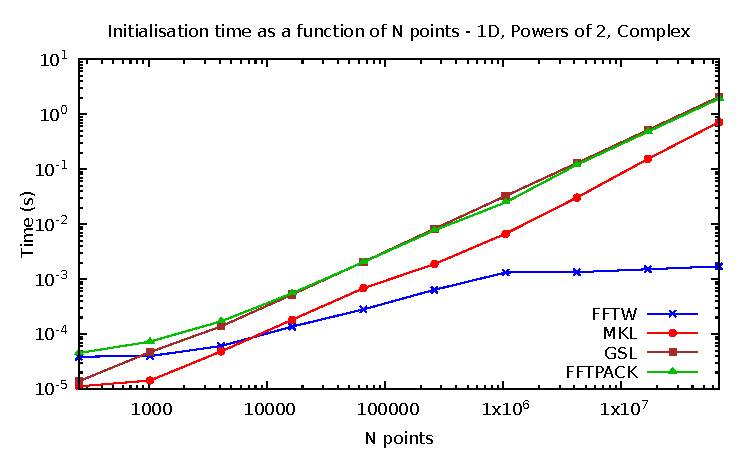
\includegraphics[width=.9\linewidth]{graphs/1d-pow2-init-c.pdf}
\caption{Intialisation (complex)}
\label{1DPOW2CI}
\end{subfigure}%
\begin{subfigure}{.5\textwidth}
\centering
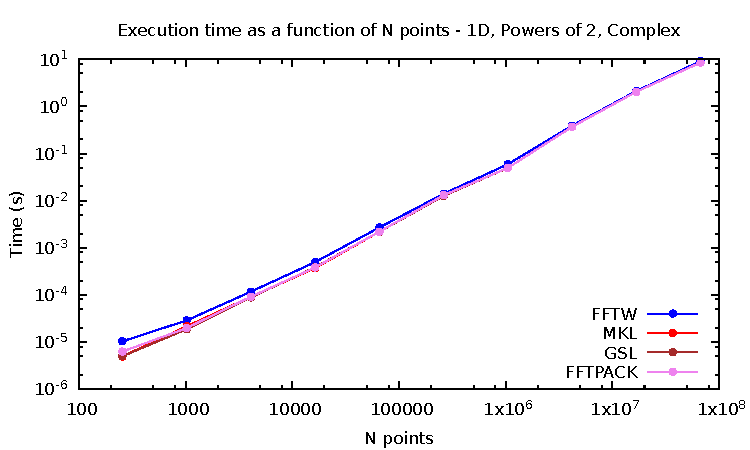
\includegraphics[width=.9\linewidth]{graphs/1d-pow2-exec-c.pdf}
\caption{Execution (complex)}
\label{1DPOW2C}
\end{subfigure}
\caption{Initialisation and execution times as a function of the number of points\\(1 dimension, powers of 2, 1 thread)}
\label{1DPOW2}
\end{figure}
\subsubsection{All the libraries}
\begin{figure}[H]
\captionsetup{width=0.8\linewidth}
\centering
\begin{subfigure}{.5\textwidth}
\centering
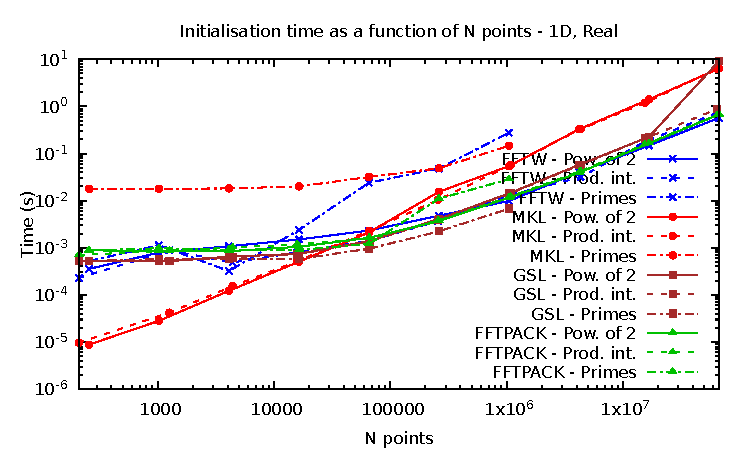
\includegraphics[width=.9\linewidth]{graphs/1d-init-r.pdf}
\caption{Intialisation (real)}
\label{1DRI}
\end{subfigure}%
\begin{subfigure}{.5\textwidth}
\centering
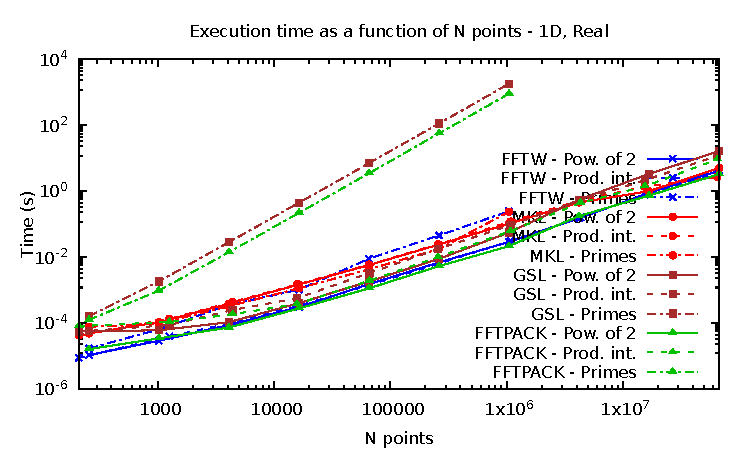
\includegraphics[width=.9\linewidth]{graphs/1d-exec-r.pdf}
\caption{Execution (real)}
\label{1DR}
\end{subfigure}\\
\begin{subfigure}{.5\textwidth}
\centering
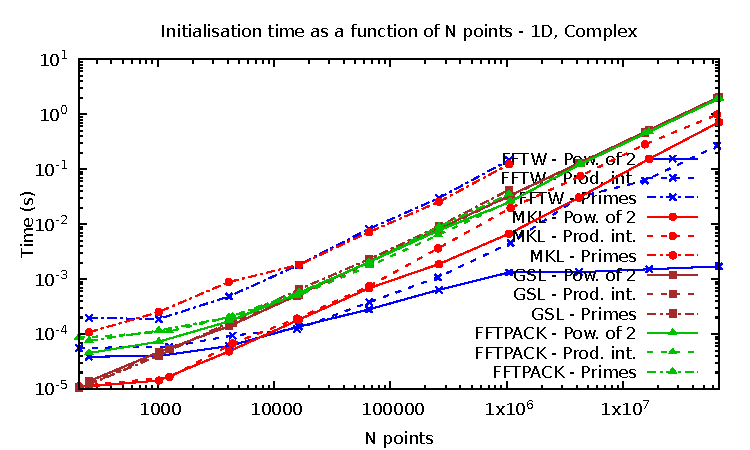
\includegraphics[width=.9\linewidth]{graphs/1d-init-c.pdf}
\caption{Intialisation (complex)}
\label{1DCI}
\end{subfigure}%
\begin{subfigure}{.5\textwidth}
\centering
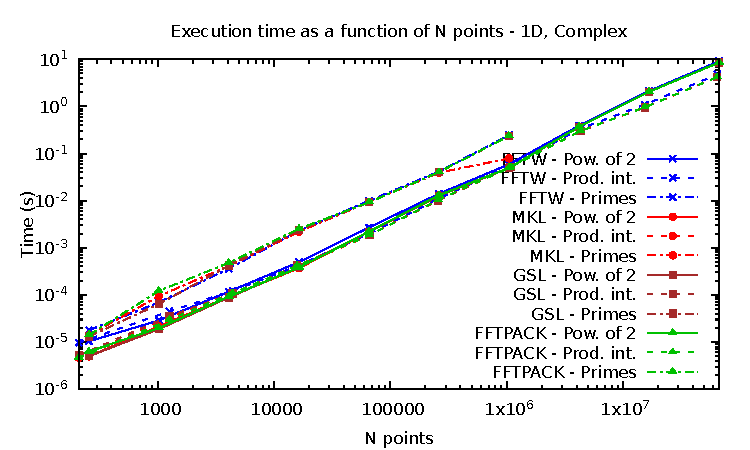
\includegraphics[width=.9\linewidth]{graphs/1d-exec-c.pdf}
\caption{Execution (complex)}
\label{1DC}
\end{subfigure}
\caption{Initialisation and execution times as a function of the number of points\\(1 dimension, 1 thread)}
\label{1D}
\end{figure}

\section{Effect of the domain size for 2D problems}\label{PERFORMANCE2D}
In this section, we measure the performance obtained in 2 dimensions, on a square domain. However, only FFTW and MKL work in these situations (Fig. \ref{2DFFTWR} - \ref{3DC}).\\
\begin{figure}[H]
\captionsetup{width=0.8\linewidth}
\centering
\begin{subfigure}{.5\textwidth}
\centering
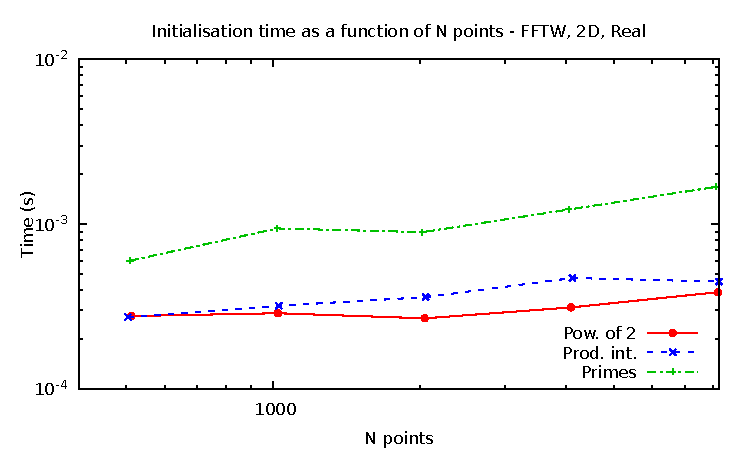
\includegraphics[width=.9\linewidth]{graphs/2d-fftw-init-r.pdf}
\caption{Intialisation (real)}
\label{2DFFTWRI}
\end{subfigure}%
\begin{subfigure}{.5\textwidth}
\centering
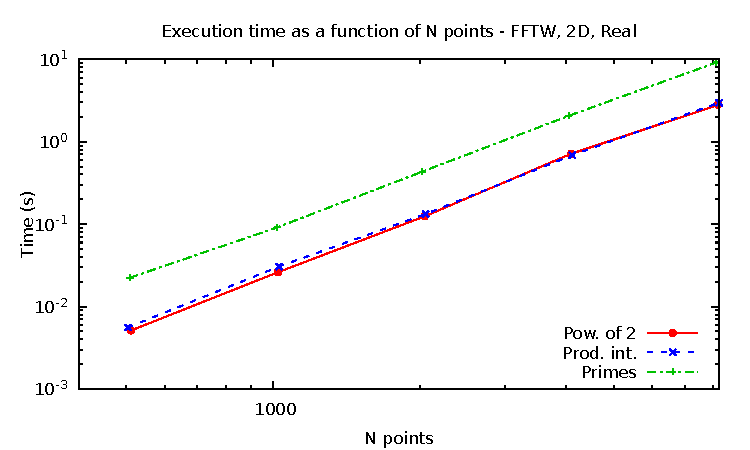
\includegraphics[width=.9\linewidth]{graphs/2d-fftw-exec-r.pdf}
\caption{Execution (real)}
\label{2DFFTWR}
\end{subfigure}\\
\begin{subfigure}{.5\textwidth}
\centering
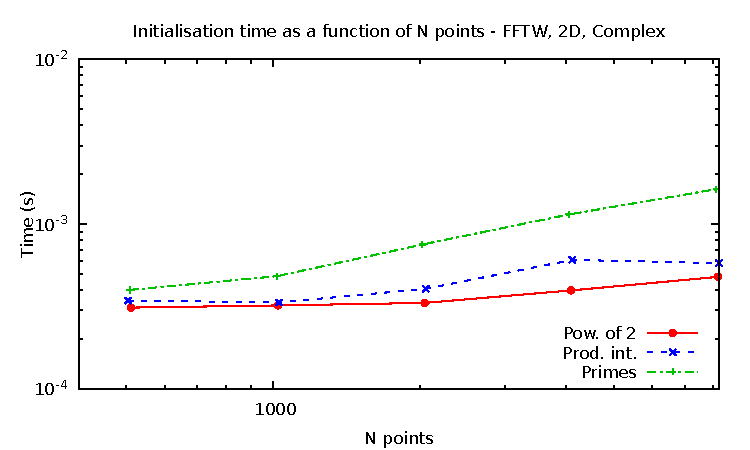
\includegraphics[width=.9\linewidth]{graphs/2d-fftw-init-c.pdf}
\caption{Intialisation (complex)}
\label{2DFFTWCI}
\end{subfigure}%
\begin{subfigure}{.5\textwidth}
\centering
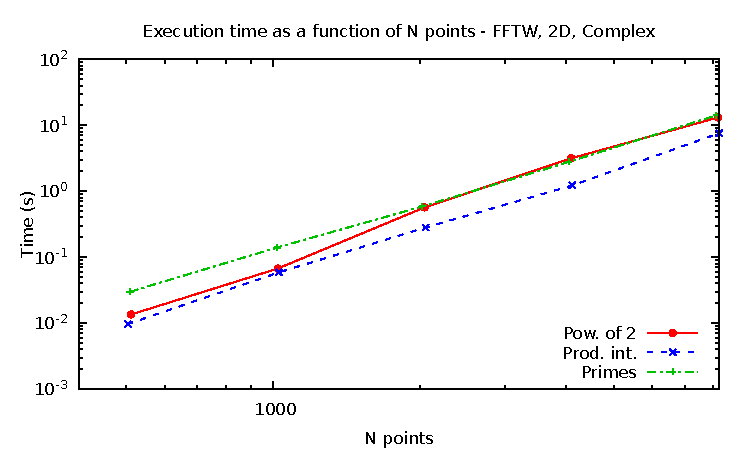
\includegraphics[width=.9\linewidth]{graphs/2d-fftw-exec-c.pdf}
\caption{Execution (complex)}
\label{2DFFTWC}
\end{subfigure}
\caption{Initialisation and execution times as a function of square side\\(2 dimensions, FFTW, 1 thread)}
\label{2DFFTW}
\end{figure}
\begin{figure}[H]
\captionsetup{width=0.8\linewidth}
\centering
\begin{subfigure}{.5\textwidth}
\centering
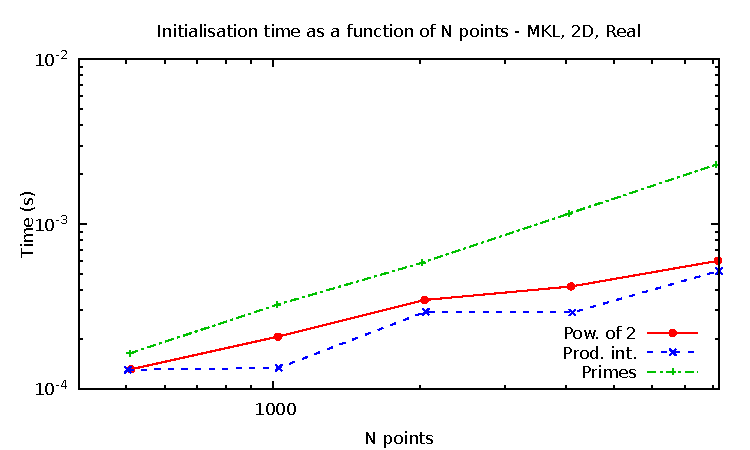
\includegraphics[width=.9\linewidth]{graphs/2d-mkl-init-r.pdf}
\caption{Intialisation (real)}
\label{2DMKLRI}
\end{subfigure}%
\begin{subfigure}{.5\textwidth}
\centering
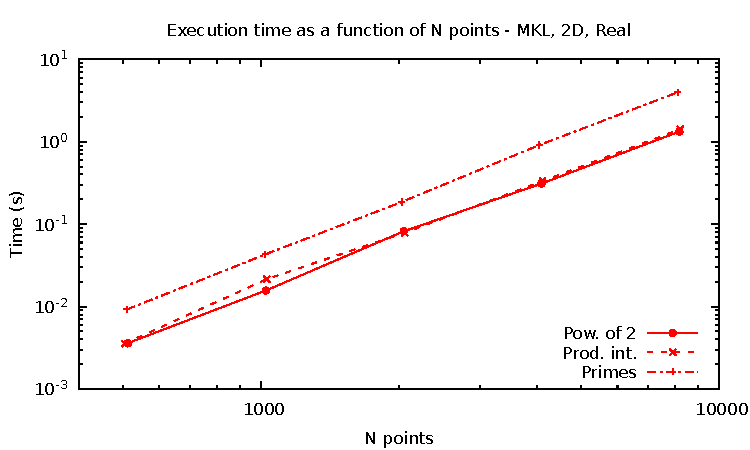
\includegraphics[width=.9\linewidth]{graphs/2d-mkl-exec-r.pdf}
\caption{Execution (real)}
\label{2DMKLR}
\end{subfigure}\\
\begin{subfigure}{.5\textwidth}
\centering
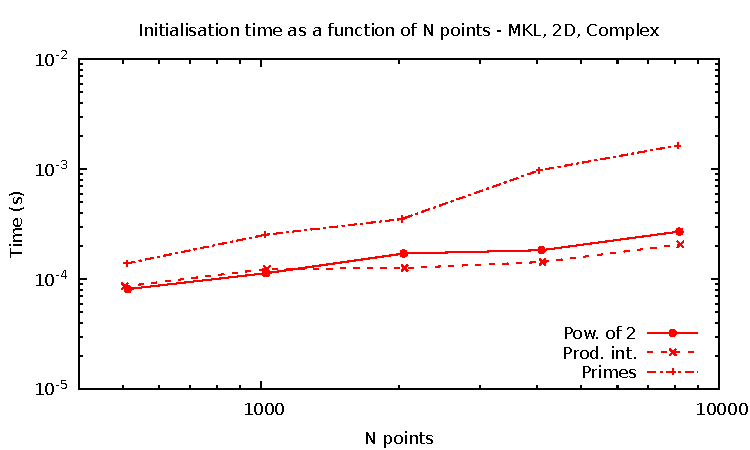
\includegraphics[width=.9\linewidth]{graphs/2d-mkl-init-c.pdf}
\caption{Intialisation (complex)}
\label{2DMKLCI}
\end{subfigure}%
\begin{subfigure}{.5\textwidth}
\centering
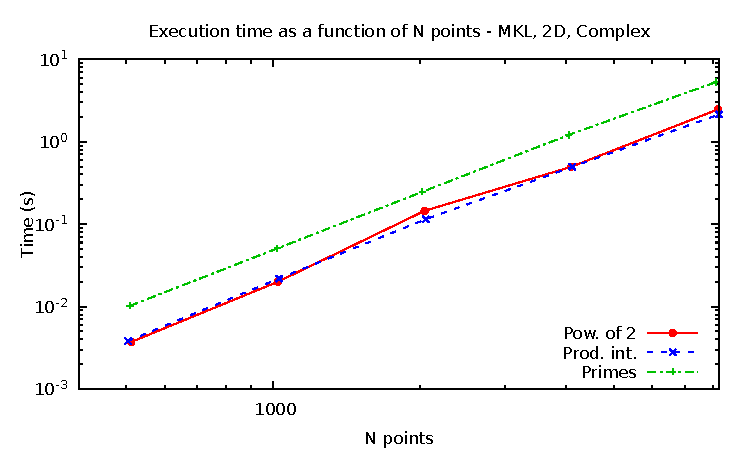
\includegraphics[width=.9\linewidth]{graphs/2d-mkl-exec-c.pdf}
\caption{Execution (complex)}
\label{2DMKLC}
\end{subfigure}
\caption{Initialisation and execution times as a function of square side\\(2 dimensions, MKL, 1 thread)}
\label{2DMKL}
\end{figure}

\begin{figure}[H]
\captionsetup{width=0.8\linewidth}
\centering
\begin{subfigure}{.5\textwidth}
\centering
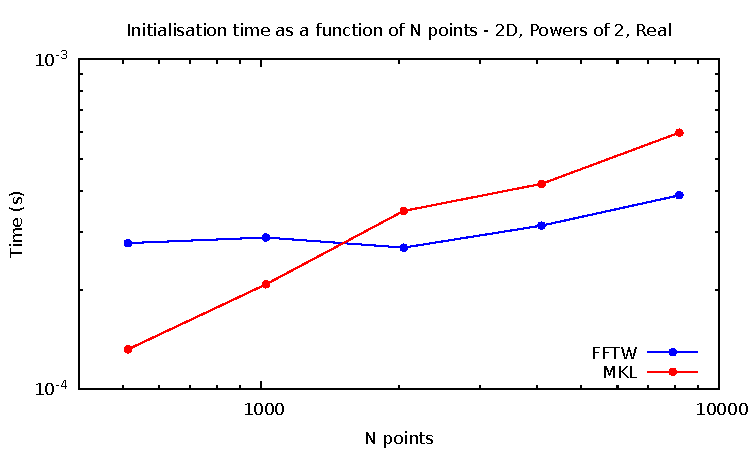
\includegraphics[width=.9\linewidth]{graphs/2d-pow2-init-r.pdf}
\caption{Intialisation (real)}
\label{2DPOW2RI}
\end{subfigure}%
\begin{subfigure}{.5\textwidth}
\centering
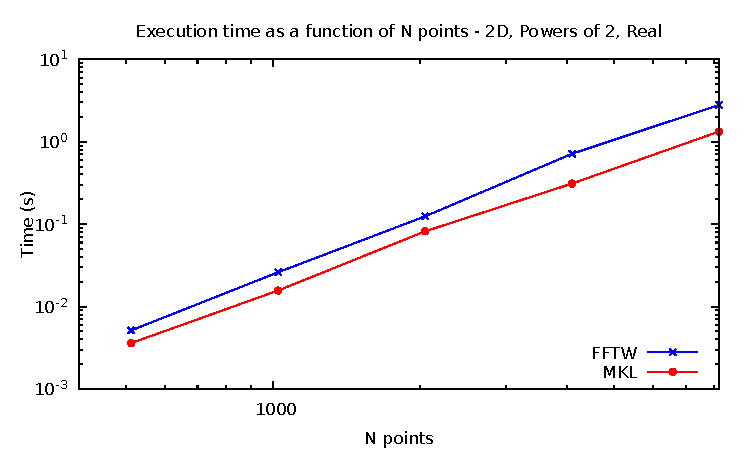
\includegraphics[width=.9\linewidth]{graphs/2d-pow2-exec-r.pdf}
\caption{Execution (real)}
\label{2DPOW2R}
\end{subfigure}\\
\begin{subfigure}{.5\textwidth}
\centering
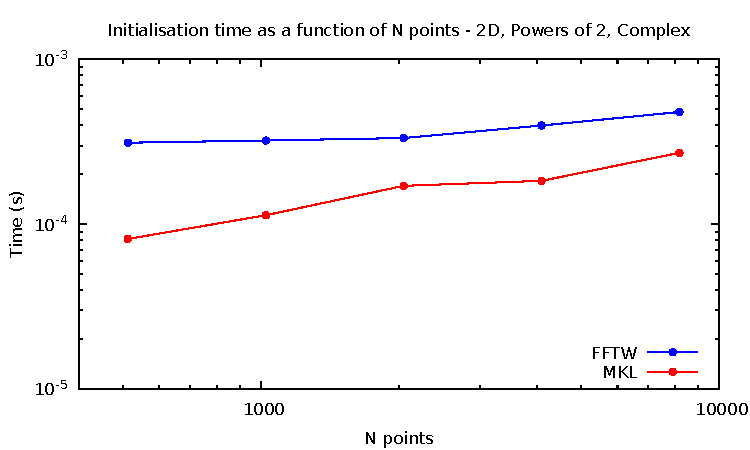
\includegraphics[width=.9\linewidth]{graphs/2d-pow2-init-c.pdf}
\caption{Intialisation (complex)}
\label{2DPOW2CI}
\end{subfigure}%
\begin{subfigure}{.5\textwidth}
\centering
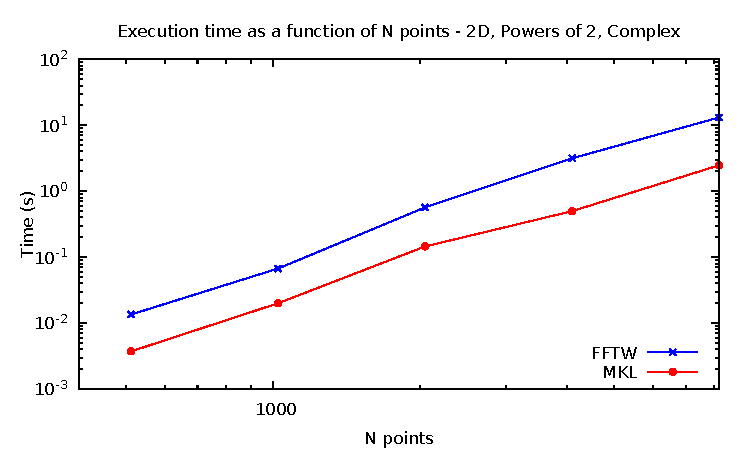
\includegraphics[width=.9\linewidth]{graphs/2d-pow2-exec-c.pdf}
\caption{Execution (complex)}
\label{2DPOW2C}
\end{subfigure}
\caption{Initialisation and execution times as a function of square side\\(2 dimensions, powers of 2, 1 thread)}
\label{2DPOW2}
\end{figure}


\begin{figure}[H]
\captionsetup{width=0.8\linewidth}
\centering
\begin{subfigure}{.5\textwidth}
\centering
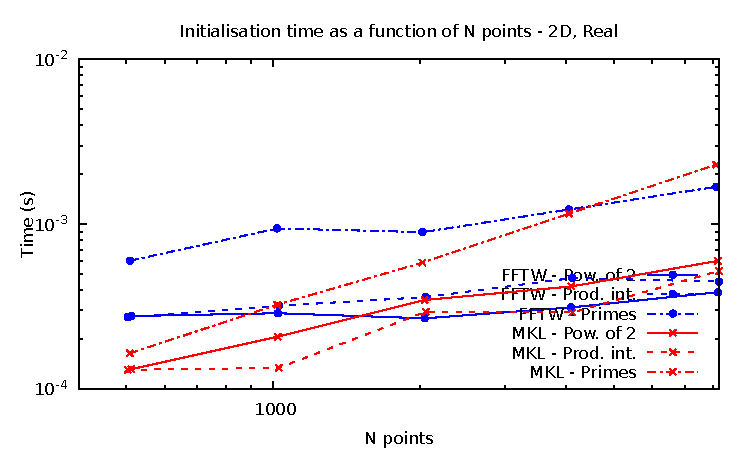
\includegraphics[width=.9\linewidth]{graphs/2d-init-r.pdf}
\caption{Intialisation (real)}
\label{2DRI}
\end{subfigure}%
\begin{subfigure}{.5\textwidth}
\centering
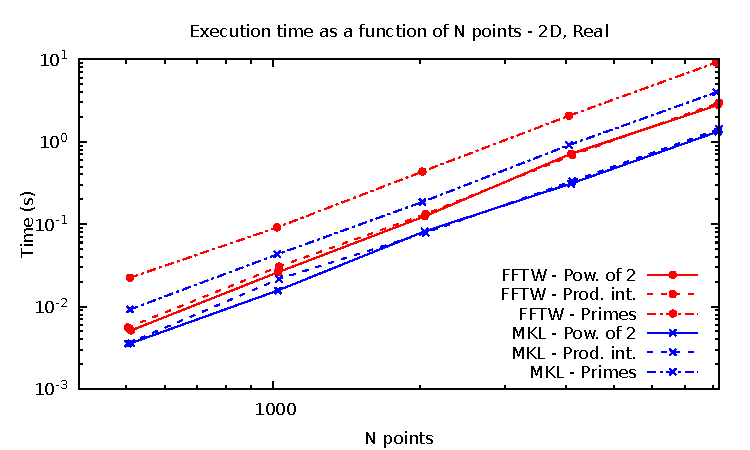
\includegraphics[width=.9\linewidth]{graphs/2d-exec-r.pdf}
\caption{Execution (real)}
\label{2DR}
\end{subfigure}\\
\begin{subfigure}{.5\textwidth}
\centering
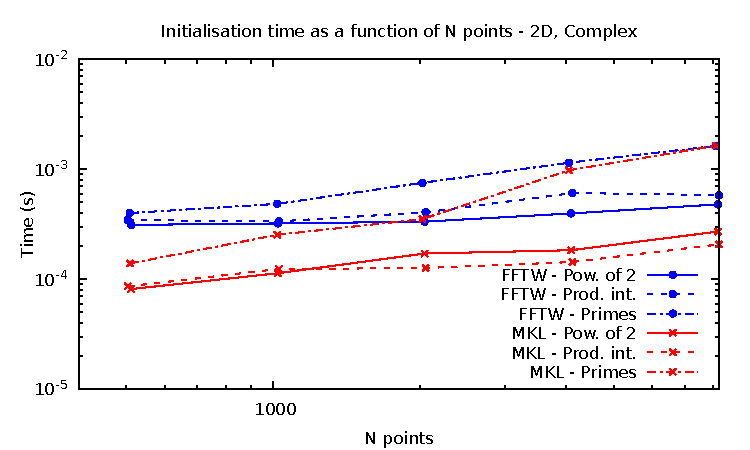
\includegraphics[width=.9\linewidth]{graphs/2d-init-c.pdf}
\caption{Intialisation (complex)}
\label{2DCI}
\end{subfigure}%
\begin{subfigure}{.5\textwidth}
\centering
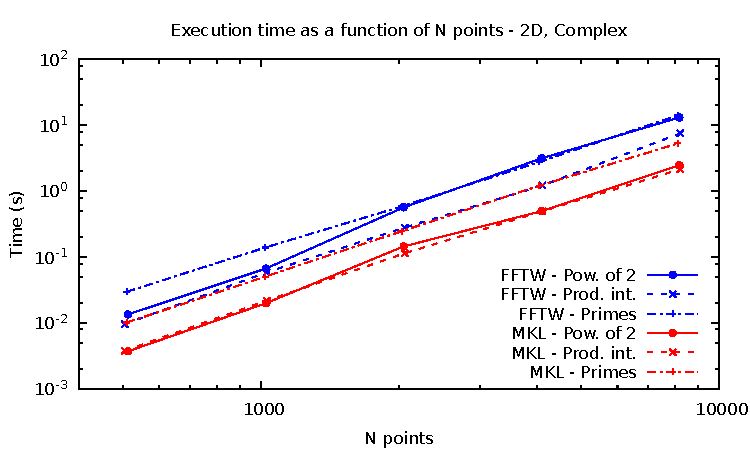
\includegraphics[width=.9\linewidth]{graphs/2d-exec-c.pdf}
\caption{Execution (complex)}
\label{2DC}
\end{subfigure}
\caption{Initialisation and execution times as a function of square side\\(2 dimensions, 1 thread)}
\label{2D}
\end{figure}

\section{Effect of the domain size for 3D problems}\label{PERFORMANCE3D}
We now study the performance measure the performance achieved in 3 dimensions, on a cubic domain, with  the FFTW and MKL libraries. So far, when working in several dimensions, we considered only domains whose sides were of equal lengths, that is a square or a cube. We will address the effect of assymetrical domains in Section \ref{FLATNESS}. 
\
\begin{figure}[H]
\captionsetup{width=0.8\linewidth}
\centering
\begin{subfigure}{.5\textwidth}
\centering
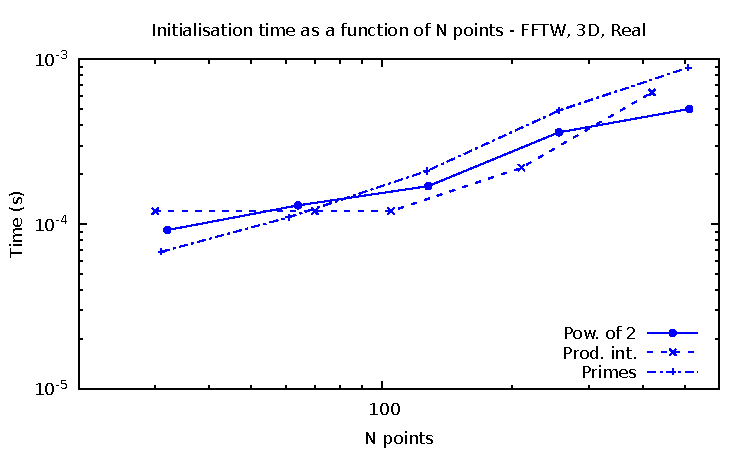
\includegraphics[width=.9\linewidth]{graphs/3d-fftw-init-r.pdf}
\caption{Intialisation (real)}
\label{3DFFTWRI}
\end{subfigure}%
\begin{subfigure}{.5\textwidth}
\centering
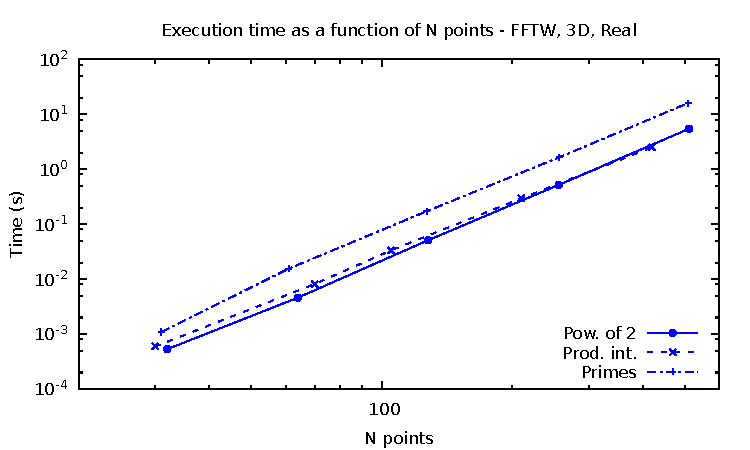
\includegraphics[width=.9\linewidth]{graphs/3d-fftw-exec-r.pdf}
\caption{Execution (real)}
\label{3DFFTWR}
\end{subfigure}\\
\begin{subfigure}{.5\textwidth}
\centering
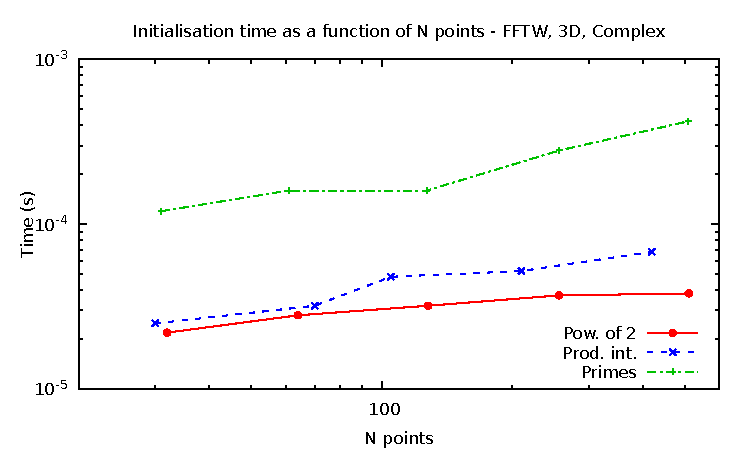
\includegraphics[width=.9\linewidth]{graphs/3d-fftw-init-c.pdf}
\caption{Intialisation (complex)}
\label{3DFFTWCI}
\end{subfigure}%
\begin{subfigure}{.5\textwidth}
\centering
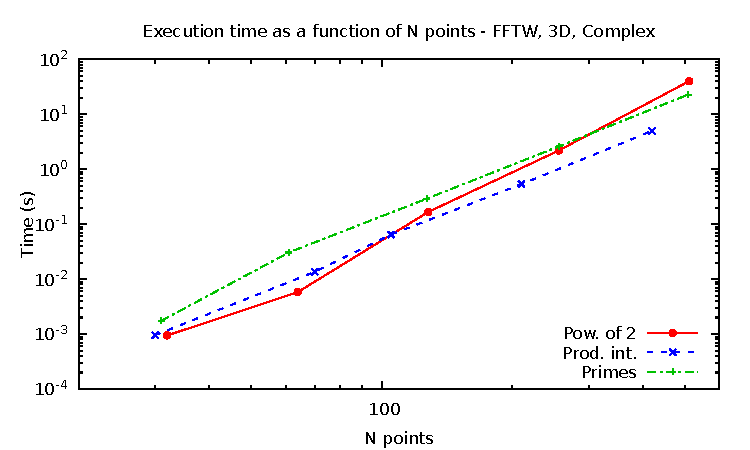
\includegraphics[width=.9\linewidth]{graphs/3d-fftw-exec-c.pdf}
\caption{Execution (complex)}
\label{3DFFTWC}
\end{subfigure}
\caption{Initialisation and execution times as a function of cube side\\(3 dimensions, FFTW, 1 thread)}
\label{3DFFTW}
\end{figure}


\begin{figure}[H]
\captionsetup{width=0.8\linewidth}
\centering
\begin{subfigure}{.5\textwidth}
\centering
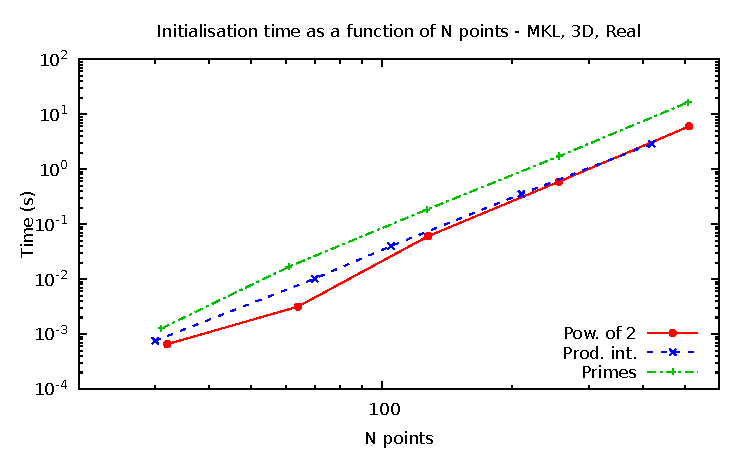
\includegraphics[width=.9\linewidth]{graphs/3d-mkl-init-r.pdf}
\caption{Intialisation (real)}
\label{3DMKLRI}
\end{subfigure}%
\begin{subfigure}{.5\textwidth}
\centering
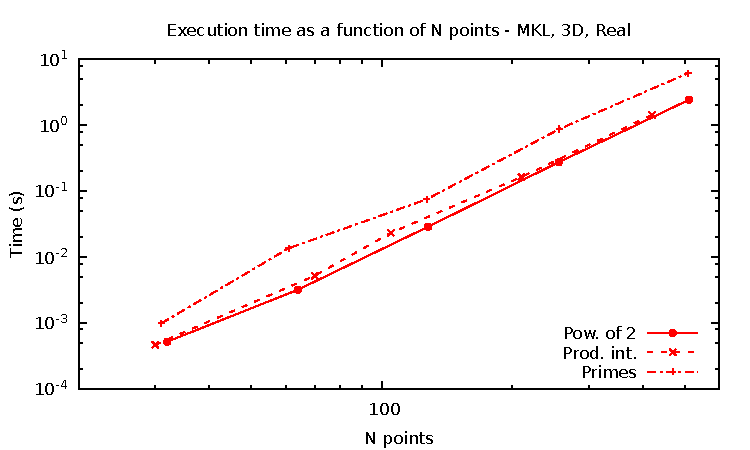
\includegraphics[width=.9\linewidth]{graphs/3d-mkl-exec-r.pdf}
\caption{Execution (real)}
\label{3DMKLR}
\end{subfigure}\\
\begin{subfigure}{.5\textwidth}
\centering
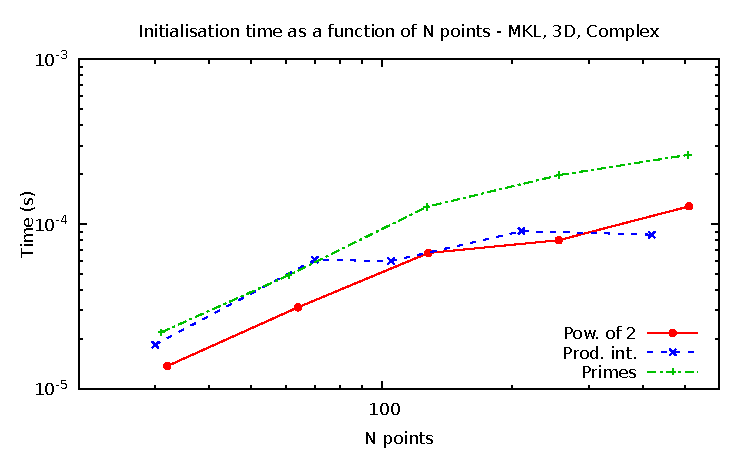
\includegraphics[width=.9\linewidth]{graphs/3d-mkl-init-c.pdf}
\caption{Intialisation (complex)}
\label{3DMKLCI}
\end{subfigure}%
\begin{subfigure}{.5\textwidth}
\centering
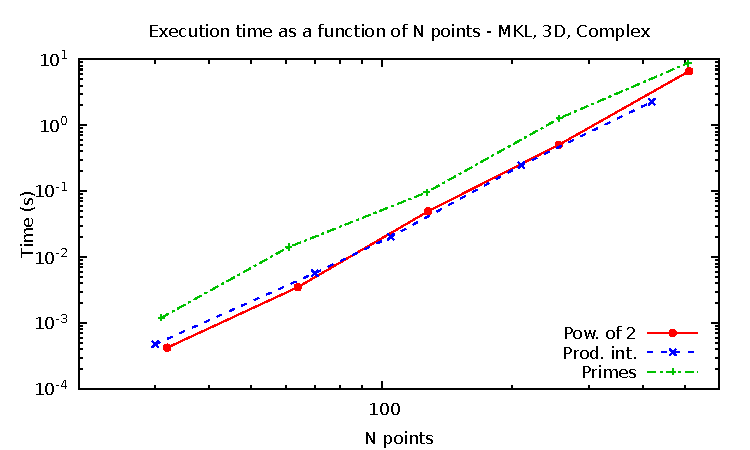
\includegraphics[width=.9\linewidth]{graphs/3d-mkl-exec-c.pdf}
\caption{Execution (complex)}
\label{3DMKLC}
\end{subfigure}
\caption{Initialisation and execution times as a function of cube side\\(3 dimensions, MKL, 1 thread)}
\label{3DMKL}
\end{figure}

\begin{figure}[H]
\captionsetup{width=0.8\linewidth}
\centering
\begin{subfigure}{.5\textwidth}
\centering
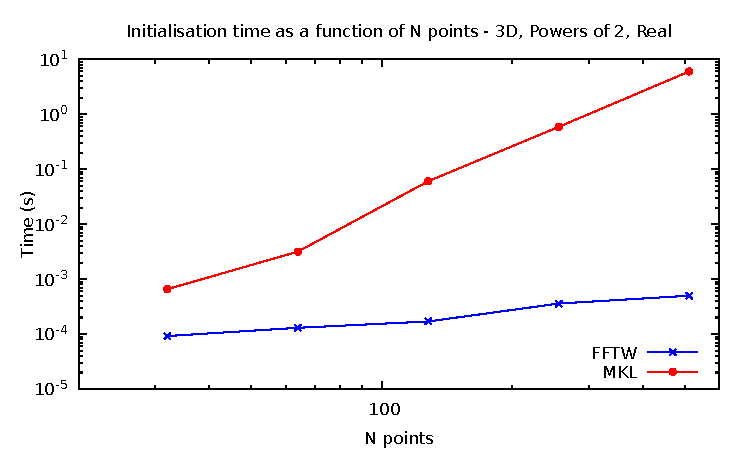
\includegraphics[width=.9\linewidth]{graphs/3d-pow2-init-r.pdf}
\caption{Intialisation (real)}
\label{3DPOW2RI}
\end{subfigure}%
\begin{subfigure}{.5\textwidth}
\centering
\includegraphics[width=.9\linewidth]{graphs/3d-pow2-exec-r.pdf}
\caption{Execution (real)}
\label{3DPOW2R}
\end{subfigure}\\
\begin{subfigure}{.5\textwidth}
\centering
\includegraphics[width=.9\linewidth]{graphs/3d-pow2-init-c.pdf}
\caption{Intialisation (complex)}
\label{3DPOW2CI}
\end{subfigure}%
\begin{subfigure}{.5\textwidth}
\centering
\includegraphics[width=.9\linewidth]{graphs/3d-pow2-exec-c.pdf}
\caption{Execution (complex)}
\label{3DPOW2C}
\end{subfigure}
\caption{Initialisation and execution times as a function of cube side\\(3 dimensions, powers of 2, 1 thread)}
\label{3DPOW2}
\end{figure}

\begin{figure}[H]
\captionsetup{width=0.8\linewidth}
\centering
\begin{subfigure}{.5\textwidth}
\centering
\includegraphics[width=.9\linewidth]{graphs/3d-init-r.pdf}
\caption{Intialisation (real)}
\label{3DRI}
\end{subfigure}%
\begin{subfigure}{.5\textwidth}
\centering
\includegraphics[width=.9\linewidth]{graphs/3d-exec-r.pdf}
\caption{Execution (real)}
\label{3DR}
\end{subfigure}\\
\begin{subfigure}{.5\textwidth}
\centering
\includegraphics[width=.9\linewidth]{graphs/3d-init-c.pdf}
\caption{Intialisation (complex)}
\label{3DCI}
\end{subfigure}%
\begin{subfigure}{.5\textwidth}
\centering
\includegraphics[width=.9\linewidth]{graphs/3d-exec-c.pdf}
\caption{Execution (complex)}
\label{3DC}
\end{subfigure}
\caption{Initialisation and execution times as a function of cube side\\(3 dimensions, 1 thread)}
\label{3D}
\end{figure}
\subsection{Flatness}\label{FLATNESS}

These experiments were carried out with domains whose dimensions were the same in all directions, that is, squares or cubes. We have observed that there is no clear trend in the way the flatness of the domain affects the performance. Fig. \ref{FLATNESS} shows the performance obtained, in 3 dimensions, for a cuboid containing $512^3$ points whose sides in the $y$ and $z$ directions have identical lengths. We hade defined the flatness as the ratio between the number of points in the $y$ and $x$ directions ($N_y/N_x,\ N_y=N_z$). We varied the proportions of the volume from $512:512:512$ till $2^{24}:2:2$.  \\

\begin{figure}[H]
\captionsetup{width=0.8\linewidth}
\centering
\begin{subfigure}{.5\textwidth}
\centering
\includegraphics[width=.9\linewidth]{graphs/flatness-r.pdf}
\caption{Real}
\label{FLATNESSR}
\end{subfigure}%
\begin{subfigure}{.5\textwidth}
\centering
\includegraphics[width=.9\linewidth]{graphs/flatness-c.pdf}
\caption{Complex}
\label{FLATNESSC}
\end{subfigure}
\caption{Execution time as a function of the flatness of the domain ($N_y/N_x$), for $N_y=N_z$ (3 dimensions, powers of 2, 1 thread)}
\label{FLATNESS}
\end{figure}


\section{Requirements from the CCP}\label{CCPPETMR}
We have also benchmarked the FFT libraries in a situation corresponding to a problem encountered by the CCP/PET-MR collaboration, by computing the transform of a series of 32 square complex images whose side consists of 256 points as well as the closest prime number (257) and product of powers of small integers ($2^23^27=252$). As in the other cases, the MKL library performs better than FFTW. None of the other libraries we have considered could be used in this situation. GSL works only in one dimension. The FORTRAN version of FFTPACK does not share that limitation. However all the C/C++ wrappers we have found offer only one-dimensional transforms. Finally FFTPACK is distributed with a licence that is less constraining than the GPL but, nevertheless, the C++ wrapper provided by CASA that we have used is distributed under the GPL v2.

\begin{figure}[H]
\captionsetup{width=0.6\textwidth}
\centering
\includegraphics[height=8cm]{graphs/ccppetmr.pdf}
\caption{Execution time for the transform of 32 complex square images as a function of square side\\(2 dimensions, complex, 1 thread)}
\label{method}
\end{figure}

\section{Acknowledgements}
The special sentence that only Barbara knows.
\begin{thebibliography}{9}

\bibitem{fftw}
Frigo, Matteo and Johnson, Steven G.,
{\it The Design and Implementation of FFTW3},
Proceedings of the IEEE,
2005,
93,
2,
216--231,
Special issue on ``Program Generation, Optimization, and Platform Adaptation''
\bibitem{mkl}
\hyperlink{https://software.intel.com/en-us/mkl}{https://software.intel.com/en-us/mkl}

\bibitem{gsl}
M. Galassi et al, {\it GNU Scientific Library Reference Manual (3rd Ed.)}, ISBN 0954612078
  
\bibitem{fftpack}
P.N. Swarztrauber, {\it Vectorizing the FFTs}, Parallel Computations (G. Rodrigue, ed.), Academic Press, 1982, pp. 51--83.
  
\bibitem{casa}
McMullin, J. P., Waters, B., Schiebel, D., Young, W., Golap, K.,
{\it Astronomical Data Analysis Software and Systems XVI},
ASP Conf. Ser. 376, ed. R. A. Shaw, F. Hill, D. J. Bell (San Francisco, CA: ASP), 127

\bibitem{code}
\hyperlink{git@github.com:SoftwareOutlook/FFTC.git}{git@github.com:SoftwareOutlook/FFTC.git}
    
\bibitem{ccppetmr}
\hyperlink{https://www.ccppetmr.ac.uk/}{https://www.ccppetmr.ac.uk/}

\bibitem{softwareoutlook}
\hyperlink{https://www.softwareoutlook.ac.uk/}{https://www.softwareoutlook.ac.uk/}

\bibitem{archer}
ARCHER: UK National Computing Service, \hyperlink{https://www.archer.ac.uk/}{https://www.archer.ac.uk/}
  
\end{thebibliography}

\end{document}
